\documentclass[report]{../../custom}
\begin{document}
\maketitle

\noindent \textbf{摘要:}
实现 SPHINCS+ 算法签名,思考优化方向。SPX 包含三个主要组件:FORS、HT 树和 WOTS+ 签名。1)FORS:通过分割哈希值生成多棵子树,计算根节点及认证路径。2)HT 树:由多层 Merkle 树组成,每层使用 WOTS+ 签名进行计算,最终得到公钥根节点。3)WOTS+ 签名:基于哈希链计算叶子节点,用于 HT 树的构建。
为提升签名速度,分析了签名过程的时间复杂度,指出 HT 阶段为主要计算瓶颈,考虑使用并行化计算以提高效率。

\vskip 0.5cm

\noindent \textbf{下周计划:} 1)GPU并行化实现FORS和HT树,2)推进论文写作。

\section{算法实现}

这周我们实现了算法签名。分析了 SPHINCS+ (SPX) 的所有组件。对于 SPX,它包含了三个主要组件。从最高层来看,SPX 接收长度为 $m$ 的消息 $msg$ 作为输入,并且在签名者一侧拥有它自己的安全密钥 $sk_{seed}$ 和公钥 $pk_{seed}$。因此,认证消息可以表示为
\[
  SPX_{sign}: (msg, sk_{seed}) \mapsto (pk_{root}, auth).
\]
首先,消息 $msg$ 会被输入到哈希函数中(具体可根据不同安全级别选择不同的哈希函数),哈希函数的输出包含一个值 $hm$,以及用于 FORS 签名和 HT(多层 XMSS 树)签名时分别需要的 $tree_{index}$。

\subsection{FORS}

哈希函数输出的 $hm$ 是长度为 $n$ 字节的值(此长度取决于特定的 SPX 版本)。接下来我们进行 FORS 签名操作:

1. 将 $8 \times n$ 比特长度的 $hm$ 根据 FORS 的树高 $t$ 分割。FORS 的叶子节点数为 $2^t$,需要满足 $t \,|\, (8 \times n)$,即 $k \times t = (8 \times n)$,其中 $k$ 是 FORS 的树数目。
2. 在每棵 FORS 子树中,叶子节点的私钥是由 $sk_{seed}$ 和其他字段随机生成的。
3. 对各私钥(由 $sk_{1 \dots k}$)用哈希函数处理,得到叶子节点,据此计算每棵子树的根节点。然后将这 $k$ 棵子树的根节点再哈希得到 $FORS_{pk}$。
注:在 FORS 中,$auth$ 是用于认证的旁枝节点,其索引由拆分后的 $hm$ 来确定(即 $k$ 个索引)。

在图~\ref{fig:fors_tree} 中可以看到一个示例 FORS 树,其中 $k=3,\, t=1$。红色节点表示公开信息,绿色节点需要验证者根据给定的公钥以及哈希链进行计算。

\begin{figure}[h!]
  \begin{center}
    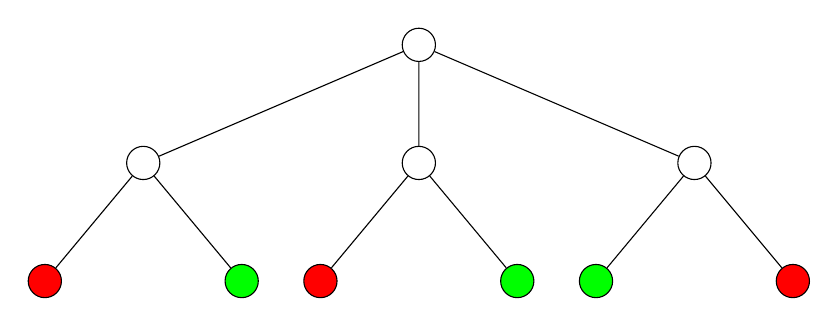
\begin{tikzpicture}[level distance=1.5cm,
        level 1/.style={sibling distance=3.5cm},
        level 2/.style={sibling distance=2.5cm},
      every node/.style={circle, draw, fill=white, inner sep=4pt, minimum size=12pt}]
      % Root node
      \node (root) [] {}
      % First level
      child {node [] {}
        % Second level
        child {node [fill=red!100] {}}
        child {node [fill=green!100] {}}
      }
      child {node [] {}
        % Second level
        child {node [fill=red!100] {}}
        child {node [fill=green!100] {}}
      }
      child {node [] {}
        % Second level
        child {node [fill=green!100] {}}
        child {node [fill=red!100] {}}
      };

    \end{tikzpicture}

  \end{center}
  \caption{FORS 树示例,这里 $k=3,t=1$。红色节点表示公开信息,绿色节点需要根据公钥校验计算。}\label{fig:fors_tree}
\end{figure}

\subsection{HT}

接着我们得到长度为 $n$ 字节的 FORS 根节点,作为 HT 计算的起点。在 FORS 中,树高为 $t$;在 HT 树中,树高记为 $h'$(即高度 - 1),其对应的认证路径需要相应的节点。与 FORS 有多棵并行的 Merkle 树不同,HT 由 $d$ 层 Merkle 树组成,每层计算后得到最终的根节点,也就是最终的公钥根节点。

在图~\ref{fig:HT_tree} 中,红色部分是认证路径节点以及最终的公钥根节点,绿色节点通过 WOTS+ 签名(基于哈希链)来计算。这里所使用的固定长度哈希链,其起始节点由 $sk_{seed}$ 生成,经过 $w$ 步哈希链得到 XMSS 树的叶子节点。

\begin{figure}[htp!]
  \begin{center}
    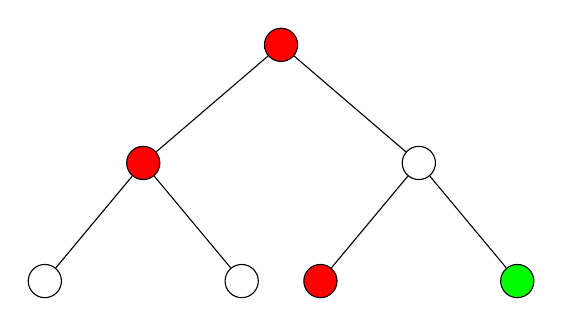
\begin{tikzpicture}[level distance=1.5cm,
        level 1/.style={sibling distance=3.5cm},
        level 2/.style={sibling distance=2.5cm},
      every node/.style={circle, draw, fill=white, inner sep=4pt, minimum size=12pt}]
      % Root node
      \node (root) [fill=red!100] {}
      % First level
      child {node [fill=red!100] {}
        % Second level
        child {node [] {}}
        child {node [] {}}
      }
      child {node [] {}
        % Second level
        child {node [fill=red!100] {}}
        child {node [fill=green!100] {}}
      };

    \end{tikzpicture}

  \end{center}
  \caption{HT 树示例,这里 $h'=1,d=2$。红色节点表示公开信息,绿色节点需要利用 FORS 根节点结合哈希链进行计算。}\label{fig:HT_tree}
\end{figure}

HT 的叶子节点由 WOTS+ 签名来计算,是 HT 计算的起点。图~\ref{fig:hashchain} 展示了 WOTS+ 签名中使用的哈希链。蓝色节点是通过 $sk_{seed}$ 生成的私有节点,哈希链长度为 $w=2$,在 FORS 签名阶段,每一位信息将映射到红色节点(对应公钥节点)。在验证阶段,验证者从红色节点出发再进行若干步哈希,得到绿色节点(也就是 XMSS 树的叶子节点)。结合图~\ref{fig:HT_tree} 中红色公开节点,就可以计算出 HT 的根节点,从而完成整个签名过程。

\begin{figure}
  \begin{center}
    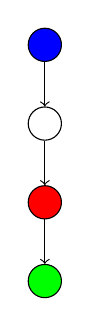
\begin{tikzpicture}[level distance=2.5cm,
      every node/.style={circle, draw, fill=white, inner sep=4pt, minimum size=12pt}]
      % Define nodes
      \node [fill=blue!100](n1) {};
      \node[below of=n1] (n2) {};
      \node[below of=n2, fill=red!100] (n3) {};
      \node[below of=n3, fill=green!100] (n4) {};

      % Connect nodes with arrows to represent the chain
      \draw[->] (n1) -- (n2);
      \draw[->] (n2) -- (n3);
      \draw[->] (n3) -- (n4);
    \end{tikzpicture}
  \end{center}
  \caption{哈希链长度示例,这里 $w=2$。蓝色节点是安全私有节点,红色节点为公开节点,绿色节点需要通过计算得到。}\label{fig:hashchain}
\end{figure}

\subsection{签名过程的实现代价分析}

现在分析签名过程在不同阶段的时间复杂度。这里假设哈希函数的计算复杂度为常数(因为 SPX 并未固定哈希函数本身,而是可以根据安全需求选用不同哈希算法)。考虑哈希函数输出长度为 $n$ 字节的情况。

\textbf{FORS 阶段:}
1) 生成叶子节点:对于每棵 FORS 子树来说,只需一次长度为 1 的哈希链。整棵树的叶子数为 $2^t$,共有 $k$ 棵树,总共需要 $2^t k$ 次哈希。
2) 计算根节点:再加上 $2^t k + 1$ 次哈希来计算得到全部 $k$ 棵子树的根节点并进一步得到 $FORS_{pk}$。其中 $2^t k = 8n$。
因此,FORS 阶段时间复杂度大约是 $16n + 1$(将 $2^t k = 8n$ 带入的近似结果)。

\textbf{WOTS+ 与 HT 阶段:}
1) 对于 WOTS+ 签名,哈希链的条数为 $n / \log w$,每条链长度为 $w$,因此一次 WOTS+ 签名需要 $n w / \log w$ 次哈希($w$ 整除 $n$)。
2) 对于一棵高度为 $h'$ 的 XMSS 树,需要计算 $2^{h'}$ 个叶子,每个叶子对应一次 WOTS+ 签名,再加上一些认证路径的计算,因此大约是 $2^{h'} (nw/\log{w} + 1)$。
如果总共有 $d$ 层 XMSS(即 HT 包含 $d$ 层),则总的 HT 计算量大约是
\[
  d \times 2^{h'} \left(\frac{n w}{\log w} + 1\right),
\]
因此,总的签名时间复杂度可以近似表示为
\[
  (16n + 1) \;+\; d \times 2^{h'} \left(\frac{n w}{\log w} + 1\right),
\]
其中,FORS 阶段对时间的贡献相对较小,而 HT 阶段占主要的计算量。

\textbf{优化思路:}
从并行计算的角度看,FORS 中有 $k$ 棵子树可以并行,但由于其计算量本身占比不大,主要的并行化需求在 HT 树中。对于 $d$ 层的 XMSS 树,可以并行地进行不同层的计算。具体来说在 SPX-128f 配置中,$k = 33,\, d = 22$,如果能够充分并行,这将显著提升签名速度。

\end{document}